\section{Corrected V3 Results and Historical Context}

\subsection{Baseline economics under the corrected model}

All 61 specified workflow steps completed, producing 330 durable artifacts
under the frozen V3 research source. The headline endpoint estimates are in
Table~\ref{tab:v3}. Full-precision values, source/output identities, endpoint
diagnostics, and the recomputed gate are retained in
\code{results/panels/btcusdt_l2_panel_v3_development_summary/summary.json}.

\begin{table}[H]
\centering
\caption{V3 baseline and primary conditional results. P\&L is an aggregate of
reset hourly episodes. The conditional interval is diagnostic.}
\label{tab:v3}
\begin{tabularx}{\textwidth}{@{}L{0.48\textwidth}YY@{}}
\toprule
Measurement & No credit, $c=0$ & Proportional, $c=1$ \\
\midrule
Mean net P\&L, USDT/window & $-0.774$ & $-0.978$ \\
95\% window-bootstrap interval & $[-1.954,+0.182]$ & $[-2.204,-0.081]$ \\
Maker fills / taker fills & 1,609 / 0 & 2,030 / 0 \\
Orders submitted & 103,871 & 104,688 \\
Cancels that arrived too late & 7 & 8 \\
30s conditional contrast, bps & $-0.456$ & $-0.064$ \\
Diagnostic clustered 95\% interval, bps & $[-1.497,+0.518]$ & $[-0.904,+0.692]$ \\
Primary endpoint screen & Blocked & Blocked \\
\bottomrule
\end{tabularx}
\end{table}

Both baseline sample means are negative. The no-credit interval crosses zero.
The proportional-credit interval lies below zero. More modeled queue
advancement produces more maker fills but does not produce a positive sample
mean. These endpoint results do not demonstrate stable profitable execution
for the locked baseline.

\begin{figure}[H]
\centering
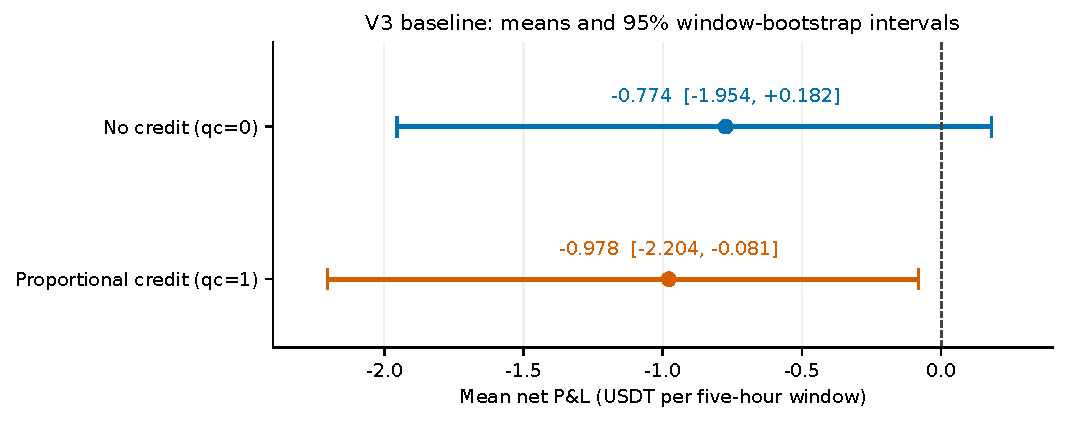
\includegraphics[width=0.93\textwidth]{figures/v3_baseline_intervals.pdf}
\caption{Current V3 mean net P\&L and 95\% window-bootstrap intervals.
Error bars resample windows.
They are not intervals for the current-minus-legacy difference.}
\label{fig:v3baseline}
\end{figure}

No selected V3 episode reports a replay gap or invalidation under the frozen
eligibility rules. Both endpoints report eight pending private actions and
four pending cancellations at the end-of-input diagnostic point, before final
expiration. Reporting those fields as zero would erase the explicit
termination boundary.

Completed-lot diagnostics also show fees matter. Mean gross and net P\&L per
matched lot are approximately $+0.002938/-0.004877$ USDT at $c=0$ and
$+0.002379/-0.005026$ USDT at $c=1$. These lot means describe completed
fragments with different sizes. They do not replace full-strategy marked
P\&L or a volume-weighted return. At a representative BTC price of 71,500
USDT, a 2 USDT half-spread is roughly 0.28 bps per side, materially smaller than
the modeled 2 bps maker fee. That arithmetic illustrates why fill quality and
fees must accompany quoting-price intuition.

\subsection{Population OFI survives the correction}

The pooled one-second normalized-OFI effect is
$+\VThreeOFIEffect$ bps per signal standard deviation, with HAC
$t=\VThreeOFITStat$, $R^2=\VThreeOFIRSquared$, and 430,259 usable
population samples. All 24 development-window coefficients are positive.
The sign, HAC, and size thresholds all pass.

The population sample is the same at both queue endpoints because queue credit
changes hypothetical execution rather than the recorded market path. The
positive pooled-coefficient prospective hypothesis therefore holds. The large
HAC statistic describes a persistent association in this sample. The low
$R^2$ and short clustered observation period prevent treating it as a broad
claim about predictable returns or deployable profits.

\subsection{The passive-fill screen fails}

At both endpoints, the rule selects the negative bucket $x<-1$ and the
nonnegative bucket $0\le x<0.25$. Their counts and mean side-aligned
30-second mid moves are:

\begin{table}[H]
\centering
\caption{The actual selected conditional buckets, pooled across buys and sells.}
\begin{tabularx}{\textwidth}{@{}L{0.16\textwidth}L{0.25\textwidth}YY@{}}
\toprule
Queue credit & Selected bucket & Maker observations & Mean move, bps \\
\midrule
$c=0$ & $x<-1$ & 685 & $-1.747$ \\
$c=0$ & $0\le x<0.25$ & 157 & $-2.203$ \\
$c=1$ & $x<-1$ & 817 & $-1.810$ \\
$c=1$ & $0\le x<0.25$ & 196 & $-1.875$ \\
\bottomrule
\end{tabularx}
\end{table}

Both selected buckets exceed the minimum count, so the endpoint result is
\code{fail_signal}, not \code{inconclusive_power}. Their contrasts,
$-0.456$ and $-0.064$ bps, are below the predeclared $+1.0$ bps bar. Neither
endpoint invokes the optional five-second fallback.

\begin{figure}[H]
\centering
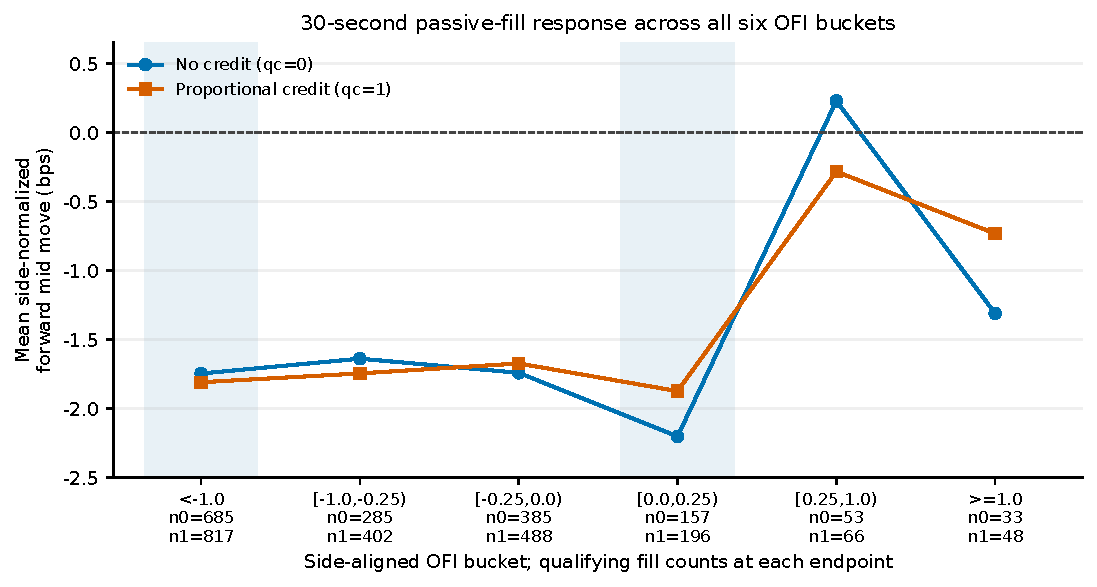
\includegraphics[width=0.98\textwidth]{figures/v3_ofi_buckets.pdf}
\caption{V3 30-second fill-conditioned response across all side-aligned
normalized-OFI buckets. Counts accompany the means. The gate selects the most
populated negative and nonnegative buckets, not the two extreme buckets. The
selected buckets are shaded blue. The full response does not support a simple
monotone interpretation.}
\label{fig:ofibuckets}
\end{figure}

Every window contributes observations to each selected bucket at both
endpoints. The clustered intervals are $[-1.497,+0.518]$ bps at $c=0$ and
$[-0.904,+0.692]$ bps at $c=1$, with no undefined resamples. They cross zero
and condition on the originally selected labels. They support reporting a
weakly separated selected comparison, without proving a universal absence of
OFI information or the profitability of an unrun transformation.

\begin{finding}
\textbf{Decision.} The combined development screen is \code{blocked}. The
baseline's passive fills do not clear the defined conditional materiality
screen despite population OFI support. No OFI-gated candidate strategy was
evaluated, no candidate parameters were tuned, and the holdout remains
strategy-sealed.
\end{finding}

\subsection{What changed relative to historical V2}

The old and current studies use the same selected development windows, but
different execution and snapshot semantics. Their no-credit mean net P\&L
changes from $-0.686$ to $-0.774$ USDT/window, a descriptive difference of
$-0.088129$. Proportional credit changes from $-1.043$ to $-0.978$, a
difference of $+0.064866$. The no-credit interval still crosses zero and the
proportional interval remains below zero. These differences are model
sensitivity, not paired confidence intervals or proof that either model is
closer to actual exchange fills.

Historical conditional OFI separation was $-0.376$ bps with no credit and
$+0.127$ bps with proportional credit. Both already failed the screen. V3
changes the numeric contrasts and execution composition while preserving the
predeclared block. The historical microprice population test also missed its
significance and size screens: its one-second effect was about 0.0190 bps per
standard deviation, with HAC $t=1.74$.

V2 additionally swept queue credit $\{0,.25,.5,.75,1\}$ at 10 ms entry
latency and the two endpoints at 0 and 50 ms. That frozen grid showed more
modeled credit increasing throughput while matched net economics worsened
from roughly $-9.75$ to $-23.65$ USDT/BTC. The intermediate-credit and latency
grid has \emph{not} been relabeled as V3: the completed current protocol covers
the two endpoints at 10 ms entry and cancellation latency. Extending that grid
would be a separate versioned experiment.

\subsection{What the evidence answers}

The corrected measurement supports both prospective statements: the pooled
OFI coefficient remains positive, and the defined conditional separation
remains below 1.0 bps with adequate selected counts at both endpoints. The
useful distinction is between a population association and the conditional
question posed by this baseline's fills. It does not establish that passive
market making is impossible, that every signal transform fails, or that a
blocked candidate would necessarily lose. Those would require additional,
separately specified experiments.
